\section{Analysis of the MPJPE when deviating from the constraints}

The original model of the 3D pose estimation system by \citet{drover18}, which is described in Section \ref{sec:network}, requires the input pose to be normalized in the following way:
\begin{enumerate}[label=(\Alph*)]
	\item The 2D input pose's root joint is centered at the origin.
	\item A designated norm limb has length 0.1.
\end{enumerate}

In reality both assumptions are rarely satisfied.
Thus \citet{drover18} normalize the input 2D poses by shifting and scaling before feeding them to the generator.
In this chapter we will see both theoretically and experimentally that this approach inevitably leads to additional errors being introduced to the system.

\Todo[inline]{Figure of camera projection}

In the following we will assume that the camera used for projection is located at the origin of the coordinate system and looks into positive z direction.
All poses are assumed to have z coordinates greater than camera's focal length $f$ in order to be projected in front of the camera.
The generator $G$ will be regarded as a black box that takes a normalized 2D pose as input and outputs the depths (the z coordinates) of the input points which then can be reprojected into three dimensional space like in Equation \eqref{eq:perspective-re-projection}.

\subsection{Shifting along one image plane axis}
\label{sec:x-shift-error}
First we will analyze assumption (A) by examining a 3D pose $P$ which is centered at the origin of the x-y-plane.
$P$ is then shifted by the vector $(dx, dy, 0)$ along the x-y-plane and projected into two dimensions.
After 2D pose has been aligned with the image plane's origin, it is re-projected into three dimensions.
The resulting 3D pose $\widetilde{P}$ will then be compared to the original 3D pose $P$ to obtain a lower bound for the MPJPE measured.

Let $P = [(X_1, Y_1, Z_1), \dotsc, (X_n, Y_n, Z_n)]$ be a 3D pose.
For simplicity we will assume that $dy = 0$, that is, the pose $P$ is only shifted along the x axis.

\subsubsection{Theoretical analysis}
Let $P_i = (X_i, Y_i, Z_i) \in P$. 
Assume $P_i$ is shifted by $dx$ along the x axis.
The x coordinate of the projected point on the image plane is
\begin{equation}
	x_i = f \frac{X_i + dx}{Z_i} = f \frac{X_i}{Z_i} + f \frac{dx}{Z_i}\ .
\end{equation}
The projected pose is then normalized by shifting all projected points along the x axis such that the root node is located in the origin of the image plane.
Let the shifted root node have coordinates $(dx, 0, Z)$.
Then each point is shifted by $- f \frac{dx}{Z}$.
That means the new x coordinate $\widetilde{x}_i$ is given by
\begin{equation}
	\widetilde{x}_i = f \frac{X_i}{Z_i} + f \frac{dx}{Z_i} - f \frac{dx}{Z} 
	= f \frac{X_i}{Z_i} + f dx (\frac{1}{Z_i} - \frac{1}{Z})
	= x_i + f dx (\frac{1}{Z_i} - \frac{1}{Z})\ .
\end{equation}
After $G$ estimates the depth $\widetilde{Z}_i$ of the point, it is reprojected into three dimensions. The resulting x coordinate is 
\begin{equation}
	\label{eq:re-projected-X}
	\widetilde{X}_i = \frac{\widetilde{x}_i}{f} \cdot \widetilde{Z}_i
	= x_i \frac{\widetilde{Z}_i}{Z_i} + dx (\frac{1}{Z_i} - \frac{1}{Z}) \widetilde{Z}_i \ .
\end{equation}
The Euclidean distance and therefore Joint Position Error of the reprojected point to the original point is given by
\begin{equation}
\label{eq:delta-d}
	\Delta d_i = \norm{ 
	\begin{pmatrix}
		\widetilde{X}_i - X_i \\
		\widetilde{Z}_i - Z_i
	\end{pmatrix}
	}_2
\end{equation}
\Todo{Think about how to formulate the "linear relationship". "With a perfect estimation of $Z_i = \widetilde{Z_i}$, one would expect..." }
With perfect estimation of $\widetilde{Z_i} = Z_i$ Equation \eqref{eq:re-projected-X} describes a linear relationship between the offset $dx$ and the Joint Position Error (JPE) $\Delta d_i$.
But since the generator's estimation of $\widetilde{Z_i}$ can vary for different offsets $dx$ and the JPE might be smaller for other $\widetilde{Z_i} \neq Z_i$, in order to obtain a correct lower bound for the Joint Position Error, we have to calculate the $\widetilde{Z_i}$ for which $\Delta d_i$ is minimal.
The function to be minimized is
\begin{align}
	\label{eq:minimum-distance}
	f(\widetilde{Z}_i) &= \left ( \widetilde{Z}_i \cdot \left( \frac{X_i}{Z_i} + dx \left( \frac{1}{Z_i} - \frac{1}{Z} \right) \right ) - X_i \right)^2 + ( \widetilde{Z}_i - Z_i ) ^2 \\
	&= \left ( \widetilde{Z}_i \cdot a - X_i \right)^2 + ( \widetilde{Z}_i - Z_i )^2 \ ,
\end{align}
where $\left( \frac{X_i}{Z_i} + dx \left( \frac{1}{Z_i} - \frac{1}{Z} \right) \right )$ has been substituted by $a$.
In order to obtain the optimal value for $\widetilde{Z}_i$, $f$ is differentiated by $\widetilde{Z}_i$:
\begin{equation}
	f'(\widetilde{Z}_i) = 2 \cdot (\widetilde{Z}_i a^2 - a X_i + \widetilde{Z}_i - Z_i)
\end{equation}
Setting this equal to zero gives
\begin{align}
	0 &= f'(\widetilde{Z}_i) \\
	\Leftrightarrow \widetilde{Z}_i & = \frac{a X_i + Z_i}{1 + a^2} \ .
\end{align}
Putting this into \eqref{eq:delta-d} yields a total minimal error of 
\begin{equation}
	\label{eq:minimum-delta-d}
	\Delta d_i = \sqrt{\frac{(a Z_i - X_i)^2}{a^2 + 1}}\
	= dx (1 -  \frac{Z_i}{Z}) \sqrt{\frac{1}{a^2 + 1}} \ .
\end{equation}

The MPJPE $\Delta d$ for the whole pose is then calculated as the mean of all $\Delta d_i$s.

In contrast to the linear relationship, for large offsets $dx$ the minimal MPJPE converges to a constant.

This result shows that even with a perfect generator, the estimated 3D poses can never be..
In fact, the effects of 2D pose normalization by shifting only vanish if $Z_i = Z$ for all $(X_i, Y_i, Z_i) \in P$; in that all joints of the pose are located in a plane parallel to the image plane.


It follows that all poses used for training and testing should have the same offsets or otherwise ambiguities are introduced to the system.
Intuition: the poses inner angles change when shifting. Shift means we see the pose more from the side.

\subsubsection{Experimental results}
	In practice, the observable error has the same approximate shape of this function, but is much smaller than the theoretical results.
	The reason for this is the scaling that is applied to the inferred poses during the evaluation of Protocol 2 (section \ref{sec:protocol2}).
	\unsure{Validate if this is really the case. Also see in what way it is proportional.}
	It appears that the average limb length of the inferred shifted poses is increasing monotonously with increasing offset $dx$.
	That means the poses are downsized by a factor $\alpha$ in all dimensions. 
	\Todo{Explain why} Therefore the actual error is $\Delta d' = \alpha \cdot \Delta d$.
	
	\begin{figure}[ht]
		
		\centering
		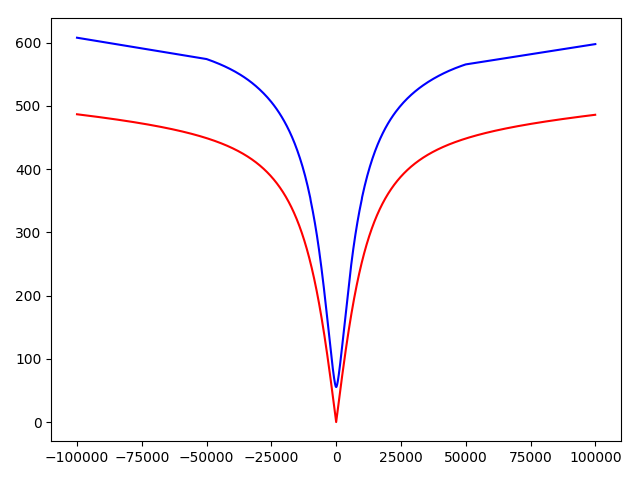
\includegraphics[scale=0.5]{images/x_shift_error.png}
		\caption{Plot of theoretical (red) and observed (blue) MPJPEs for different values of $dx$. 
			The theoretical errors are obtained by calculating the mean of the per pose errors $\alpha \Delta d$ for the evaluation data.}
		\Todo[inline]{Add axes titles, use proper image.
		use pgfplots to plot data}
		\label{fig:x-shift-error}
	\end{figure}

	It is noticeable that the performance of the network is not worse than the theoretical results by a constant offset.
	For small deviations along the x axis the network seems to be able to compensate the error introduced by shifting.
	As $dx$ increases, so does the offset between the observed and the theoretical results until it seems to converge to a constant.
	This motivates adjusting not only how the inferred points are reprojected into three dimensions but also the input the network receives.
	This will be discussed further in section \ref{sec:network-adjusting}.
	
	As shown in section \ref{sec:data-results} the MPJPE for the original 2D poses is about \Todo{Check this number} 30mm higher than the one for the synthetically generated data.
	The simplest explanation for this is that the original 2D poses do not fulfill the constraints for the system.
	The camera is not centered on the root joint and also the camera distance is most certainly not exactly ten times the length of the norm limb.
	
	Numbers: ...
	
\subsection{Shifting along the z axis}
\label{sec:z-shift-error}
\subsubsection{Theoretical analysis}
Again consider a point $P_i=(X_i, Y_i, Z_i) \in \mathbb{R}^3$. Assume that $P_i$ is shifted by $dz$ along the z axis.
The x coordinate of the projected point on the image plane is
\begin{equation}
	x_i = f \frac{X_i}{Z_i + dz}
\end{equation}
The projected points are now scaled in a way that they have the same (arbitrary) scale.  Let $\alpha$ be the scale of the set of the original projected points and $\beta$ the one of the set of shifted projected points. The scaled projected point is given by

\begin{equation}
		\widetilde{x}_i = x_i \cdot \frac{\alpha}{\beta} 
		= f \frac{Z_i}{Z_i + dz}\cdot \frac{\alpha}{\beta} 
\end{equation}
After the system estimates the depth $\widetilde{Z}_i$ of each point, they are reprojected into 3 dimensional space.
The reprojected points are given by
\begin{equation}
	\widetilde{X}_i = \frac{\widetilde{x}_i}{f} \cdot \widetilde{Z}_i
	= \frac{X_i}{Z_i + dz}\cdot \frac{\alpha}{\beta}  \cdot \widetilde{Z}_i
\end{equation}
Again we want to minimize equation \eqref{eq:delta-d}.
If we define $a := \frac{X_i}{Z_i + dz}\cdot \frac{\alpha}{\beta}$, the minimal value for $\Delta d$ is the same as in equation \eqref{eq:minimum-delta-d}.


\subsubsection{Experimental results}
	This phenomenon is also affecting our ground truth data. The poses are all projected with a camera distance $ \text{length-of-norm-limb} \cdot 10$. 
	That means the length of the projected norm limb is not exactly $0.1$ but a bit smaller or bigger. 
	Like in the discussed above those projected poses are then normalized. 
	The system estimates the depths of the normalized pose and re-projects it assuming a perfect perspective projection. 
	It therefore does not consider the effect of small deviations in z direction.
	A way to fix this would be to calculate the perfect camera distance for each pose individually before projecting them onto the image plane.
	This is not very realistic though since one might be able to determine the camera's distance to a human approximately, but definitely not exactly. This phenomenon therefore is kind of inevitable.


\subsection{Alternation of the focal length}
No difference

